\documentclass{standalone}
\usepackage{tikz,ctex}
\usepackage{tikz-3dplot} % 2-1
\usepackage{unicode-math} % 2-5,4-1,4-2
\setmathfont{Fira Math Regular}
\setmainfont{Fira Sans}
\definecolor{background}{RGB}{239, 239, 239} % 4-5,6-2,6-5
\begin{document}
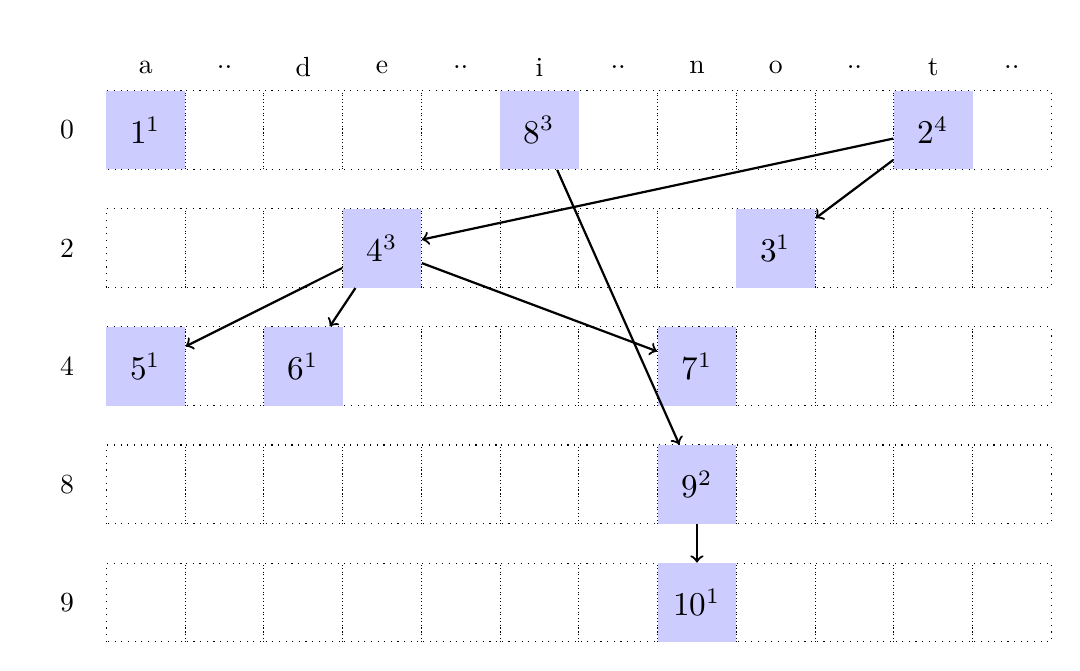
\begin{tikzpicture}[every node/.style ={rectangle,minimum width=1cm, minimum height=1cm}]
\foreach \x in {0,...,11}
\foreach \y in {0,...,4}{
    \draw[thin,dotted] (\x-.5,1.5*\y-.5) rectangle (\x+.5,1.5*\y+.5);}
\foreach \x/\y\pos/\num in {0/4/1/1,10/4/2/4,8/3/3/1,3/3/4/3,0/2/5/1,2/2/6/1,7/2/7/1,5/4/8/3,7/1/9/2,7/0/10/1}{
    \node(\pos)[fill=blue!20,font=\large] at (\x,1.5*\y) {$\pos^\num$};}   
\foreach \x/\text in{0/a,1/..,2/d,3/e,4/..,5/i,6/..,7/n,8/o,9/..,10/t,11/..}{
    \node at (\x,6.8){\text};}
\foreach \y\text in{0/9,1/8,2/4,3/2,4/0}{
    \node at (-1,1.5*\y){\text};}
\foreach \u/\v in{8/9,9/10,2/3,2/4,4/5,4/6,4/7}{
    \draw[->,thick] (\u)--(\v);}
\end{tikzpicture} 
\end{document}